% !TEX encoding = UTF-8 Unicode
% !TEX root = ../main.tex

\chapter{Bayesian Inference}
\minitoc

A common and useful conceptualization in statistics is to think data is 
generated from some true probability distribution with unknown parameters. 
Then, \emph{inference} is the process of finding out the values of those parameters 
using just a sample (also known as a dataset) from the true probability 
distribution. \citep[pp. 12]{Martin:2018aa}

\citep{Gelman2013}

Bayesian modelling can be summarized in three steps \citep{Martin:2018aa}:
\begin{enumerate}
    \item Given some data and some assumptions on how this data could 
    have been generated, design a model by combining building blocks known
     as probability distributions. Most of the time these models are crude 
     approximations, but most of the time is all we need.

     \item Use Bayes' theorem to add data to the models and derive the 
     logical consequences of combining the data and assumptions. This step
     is called conditioning the model on the data.

     \item Criticize the model by checking whether the model makes 
     sense according to different criteria, including the data, the 
     expertise on the subject, and sometimes by comparing several models.
\end{enumerate}

Bayesian models are also known as probabilistic models because they are built
 using probabilities. Why probabilities? Because probabilities are the correct
  mathematical tool to model uncertainty, so let's take a walk through the garden
   of forking paths.

Initial definitions:
\begin{description}
    \item[$p(x)$] is called as \emph{prior}\index{prior}. The prior distribution should reflect 
    what we know about the value of the parameter before seeing the data, $y$.

    \item[$p(x|\theta)$] is called as \emph{likelihood}. The likelihood is how 
    we will introduce data in our analysis. It is an expression of the 
    plausibility of the data given the parameters. In some texts, you will 
    find people call this term sampling model, statistical model, or just model.

    \item[$p(\theta|x)$] is called as \emph{posterior}. The posterior distribution 
    is the result of the Bayesian analysis and reflects all that we know about a 
    problem (given our data and model). The posterior is a probability distribution 
    for the parameters in our model and not a single value. This distribution is 
    a balance between the prior and the likelihood.

    \item[$p(\theta)$] is called as \emph{marginal likelihood}. The last term is 
    the marginal likelihood, also known as evidence. Formally, the marginal 
    likelihood is the probability of observing the data averaged over all the possible 
    values the parameters can take (as prescribed by the prior).
\end{description}

\begin{example}[Flipping a coin, {\citep[pp. 21]{Martin:2018aa}}]
    In this example, the question to be answered is: Is a coin unbiased? 

    To proceed, the following notation is defined
    \begin{description}
        \item[$\theta$] is the parameter.
        \item[$N$] is the number of tosses.
        \item[$y$] is the number of heads. 
    \end{description}

    \paragraph{Choosing the Likelihood}. Assume that only heads and tails are possible event outcomes, and that coin tosses are independent of each other. Under these assumptions, a candidate for likelihood function is the \emph{binomial} distribution:
    \begin{equation}
        p(y|\theta, N)=\dfrac{N!}{y!(N-y)!}\theta^y(1-\theta)^{N-y}\;.
    \end{equation}
    This is a discrete distribution returning the probability of getting $y$ heads 
    (or in general, successes) out of $N$ coin tosses (or in general, trials or experiments) 
    given a fixed value of $\theta$.

    The binomial distribution is a reasonable choice for the likelihood. One can see that $\theta$
    indicates how likely it is to obtain a head when tossing a coin. Since the value of $\theta$ is
    unknown, it will be obtained using Bayes' theorem.

    \paragraph{Choosing the Prior}. The prior chosen is the \emph{beta} distribution
    \begin{equation}
        p(\theta)=\dfrac{\Gamma(\alpha+|beta)}{\Gamma(\alpha)\Gamma(\beta)}\theta^{\alpha-1}(1-\theta)^{\beta-1}\;.
    \end{equation}
    The beta distribution looks similar to the binomial except for the first term which is a normalizing constant that ensures the distribution integrates to 1, and $\Gamma$ is the \emph{gamma function}.

    Why using the beta distribution as the prior? 
    \begin{itemize}
        \item The beta distribution is restricted to be between 0 and 1, in the same way parameter $\theta$ is. 
        \item The beta distribution is the conjugate prior of the binomial distribution (which we are using as the likelihood). A conjugate prior of a likelihood is a prior that, when used in combination with a given likelihood, returns a posterior with the same functional form as the prior.
    \end{itemize}
    
    \textbf{Getting the Posterior}. From  Bayes' theorem, the posterior is proportional to the likelihood times the prior:
    \begin{equation}\label{eq:tossing coin example}
        \begin{aligned}
            p(\theta|y)\propto&\ p(y|\theta)p(\theta)\\
                       =&\ \dfrac{N!}{y!(N-y)!}\theta^y(1-\theta)^{N-y}\dfrac{\Gamma(\alpha+|beta)}{\Gamma(\alpha)\Gamma(\beta)}\theta^{\alpha-1}(1-\theta)^{\beta-1}\\
                       =&\ \theta^{y+\alpha-1}(1-\theta)^{N-y+\beta-1}
        \end{aligned}
    \end{equation}
    This expression has the same functional form of a beta distribution (except for the normalization term) with $\alpha_{posterior}=\alpha_{prior}+y$ and $\beta_{posterior}=\beta_{prior}+N-y$. In fact,
    \[p(\theta|y)\propto Beta(\alpha_{prior}+y, \beta_{prior}+N-y)\;.\]

    \paragraph{Computing and Plotting the posterior.} 

    \begin{figure*}
        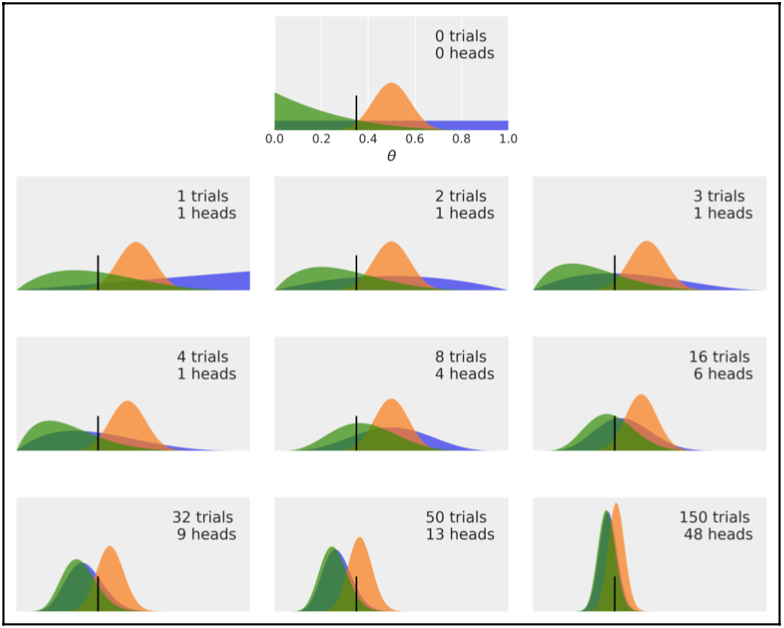
\includegraphics[width=0.9\textwidth]{prior_posteriors.png}
        \caption{Plot of \cref{eq:tossing coin example} for beta distribution parameters $(1, 1), (20, 20)$, and $(1, 4)$.}
        \label{fig:plot of posterior distributions}
    \end{figure*}

    \Cref{fig:plot of posterior distributions} plots the distribution of the posterior for three choices of the parameters of the beta distribution: $(1, 1), (20, 20)$, and $(1, 4)$.

    When, there has been 0 trials (and 0 heads), the curves plotted are the priors:
    \begin{itemize}
        \item The uniform (blue) prior represents all the possible values for the bias being equally probable a priori.
        
        \item The Gaussian-like (orange) prior is centered and concentrated around 0.5, so this prior is compatible with information indicating that the coin has more or less about the same chance of landing heads or tails.
        
        \item The skewed (green) prior puts the most weight on a tail-biased outcome.
    \end{itemize}

    The remaining subplots show posterior distributions for successive trials. The number of trials (or coin tosses) and the number of heads are indicated in each subplot's legend. There is also a black vertical line at 0.35 representing the true value for $\theta$. In practice, however, the value of $\theta$ is unknown.

    \paragraph{Conclusion.} This exercise illustrates key points of Bayesian analysis:
    \begin{itemize}
        \item The result of a Bayesian analysis is a posterior distribution, not a single value but a distribution of plausible values given the data and our model.
        
        \item The most probable value is given by the mode of the posterior (the peak of the distribution).
        
        \item The spread of the posterior is proportional to the uncertainty about the value of a parameter; the more spread out the distribution, the less certain we are.
        
        \item Intuitively, we are more confident in a result when we have observed more data supporting that result. Thus, even when numerically $\tfrac{1}{2}=\tfrac{4}{8}$, seeing four heads out of eight trials gives us more confidence that the bias is 0.5 than observing one head out of two trials. This intuition is reflected in the posterior, as you can check for yourself if you pay attention to the (blue) posterior in the third and sixth subplots; while the mode is the same, the spread (uncertainty) is larger in the third subplot than in the sixth subplot.
        
        \item Given a sufficiently large amount of data, two or more Bayesian models with different priors will tend to converge to the same result. In the limit of infinite data, no matter which prior we use, all of them will provide the same posterior. Remember that infinite is a limit and not a number, so from a practical point of view, we could get practically indistinguishably posteriors for a finite and rather small number of data points.
        
        \item How fast posteriors converge to the same distribution depends on the data and the model. In the preceding figure, we can see that the posteriors coming from the blue prior (uniform) and green prior (biased towards tails) converge faster to almost the same distribution, while it takes longer for the orange posterior (the one coming from the concentrated prior). In fact, even after 150 trials, it is somehow easy to recognize the orange posterior as a different distribution from the two others.
        
        \item Something not obvious from the figure is that we will get the same result if we update the posterior sequentially than if we do it all at once. We can compute the posterior 150 times, each time adding one more observation and using the obtained posterior as the new prior, or we can just compute one posterior for the 150 tosses at once. The result will be exactly the same. This feature not only makes perfect sense, it also leads to a natural way of updating our estimations when we get new data, a situation common in many data-analysis problems.\qedhere
    \end{itemize}
        

\end{example}

\section{Probability Theory}

\section{General Probability Model}

\subsection{Choosing the Likelihood}

\clearpage
\printbibliography[segment=\therefsegment,heading=subbibintoc]